\documentclass[11pt,a4paper]{article}

% ----------------- Idioma y fuentes -----------------
\usepackage[utf8]{inputenc}
\usepackage[T1]{fontenc}
\usepackage[spanish,es-noshorthands]{babel} % es-noshorthands: evita conflictos con listings
\usepackage{lmodern}
\usepackage{microtype}

% ----------------- Layout -----------------
\usepackage[a4paper,margin=2.3cm]{geometry}
\usepackage{parskip}
\usepackage{booktabs}
\usepackage{array}
\usepackage{longtable}
\usepackage{graphicx}
\usepackage{float}
\usepackage{enumitem}
\setlist{itemsep=2pt,topsep=3pt}

% ----------------- Colores y cajas -----------------
\usepackage{xcolor}
\definecolor{kwblue}{RGB}{0,90,180}
\definecolor{commentgreen}{RGB}{0,130,70}
\definecolor{stringred}{RGB}{170,55,45}
\definecolor{codebg}{RGB}{248,248,248}
\definecolor{rulegray}{RGB}{200,200,200}
\definecolor{accent}{RGB}{30,80,150}

\usepackage[most]{tcolorbox}
\newtcolorbox{nota}[1][Idea clave]{colback=blue!4,colframe=accent,fonttitle=\bfseries,
  title=#1,boxrule=0.6pt,arc=2pt,left=4pt,right=4pt,top=3pt,bottom=3pt}
\newtcolorbox{ojo}[1][Atencion]{colback=red!4,colframe=red!60!black,fonttitle=\bfseries,
  title=#1,boxrule=0.6pt,arc=2pt,left=4pt,right=4pt,top=3pt,bottom=3pt}

% ----------------- Listings (codigo) -----------------
\usepackage{listings}
\lstdefinestyle{py}{
  language=Python,
  basicstyle=\ttfamily\small,
  keywordstyle=\color{kwblue}\bfseries,
  commentstyle=\color{commentgreen}\itshape,
  stringstyle=\color{stringred},
  numbers=left, numberstyle=\tiny\color{gray}, numbersep=7pt,
  frame=single, framerule=0.4pt, rulecolor=\color{rulegray},
  backgroundcolor=\color{codebg},
  breaklines=true, breakatwhitespace=true, postbreak=\mbox{\textcolor{gray}{$\hookrightarrow$}\space},
  showstringspaces=false, tabsize=4, columns=fullflexible, keepspaces=true,
  captionpos=b, aboveskip=8pt, belowskip=8pt, xleftmargin=14pt,
  morekeywords={self,cls,True,False,None,as,with,assert,yield,lambda},
}
\lstset{style=py}
\newcommand{\code}[1]{\lstinline[basicstyle=\ttfamily\normalsize]|#1|}

% ----------------- Encabezados -----------------
\usepackage{fancyhdr}
\pagestyle{fancy}\fancyhf{}
\lhead{\small Auto Autonomo IAS --- Documentacion tecnica}
\rhead{\small\thepage}
\renewcommand{\headrulewidth}{0.3pt}

% ----------------- hyperref (ultimo) -----------------
\usepackage[colorlinks=true,linkcolor=accent,urlcolor=accent,citecolor=accent]{hyperref}

\title{\vspace{-1cm}\textbf{\Huge Auto Autónomo a Escala}\\[4pt]
\Large Documentación técnica completa del pipeline de \emph{Imagen $\rightarrow$ Acción}\\[10pt]
\normalsize Proyecto Integrador --- Inteligencia Artificial (ENIB)}
\author{}
\date{\today}

\begin{document}
\maketitle
\thispagestyle{empty}

\begin{abstract}
\noindent Este documento explica, \textbf{de lo general a lo particular y función por función},
todo el software del proyecto: el modelo aprende a manejar un auto a escala prediciendo, a partir
de una sola imagen de su cámara frontal, qué hacer con cada motor. Se cubre el panorama conceptual
(qué se quiere, qué hardware hay, qué datos tenemos y sus limitaciones), el \textbf{pipeline de datos}
(de los \texttt{labels.csv} crudos a los CSV que consume la red), los \textbf{cuatro motores de modelo}
(per-frame, temporal, con signo e híbrido), los \textbf{entrypoints} que congelan cada experimento, y
la \textbf{herramienta de exploración de hiperparámetros}. Cada bloque incluye el código fuente completo
y una explicación detallada. El hilo conductor del proyecto es una conclusión honesta: \emph{con los datos
disponibles, ninguna arquitectura sofisticada supera a un modelo per-frame simple; el techo es el dato.}
\end{abstract}

\tableofcontents
\newpage

% =====================================================================
\part{Contexto: qué problema resolvemos}
% =====================================================================

\section{El objetivo en una frase}
Dada una \textbf{imagen} de la cámara frontal de un auto a escala, queremos predecir la \textbf{acción de
manejo}: qué hacer con el motor izquierdo y con el derecho. Es \textbf{aprendizaje supervisado}
(\emph{imagen $\rightarrow$ acción}), un laboratorio de visión por computadora + toma de decisiones.
\textbf{No es aprendizaje por refuerzo}: no hay recompensas ni exploración; tenemos grabaciones de un
piloto humano manejando, y el modelo aprende a imitarlo.

\begin{nota}[El marco mental]
Pensá en cada frame como una pregunta tipo examen: ``dada esta foto, ¿qué hizo el piloto?''. La respuesta
correcta (la etiqueta) es el comando que el piloto envió a los motores en ese instante. Entrenar = mostrarle
miles de pares (foto, comando) y ajustar la red para que sus predicciones se parezcan a lo que hizo el humano.
\end{nota}

\section{El hardware y la física del problema}
El auto es una Raspberry Pi 4 + un driver de motores \textbf{L298N} + una webcam. \textbf{No hay encoders ni
sensores de velocidad}: lo único que se registra es lo que el piloto \emph{ordenó}, no lo que el auto
\emph{midió}. Esto es central para entender las etiquetas.

\begin{itemize}
  \item \textbf{\code{speedA} / \code{speedB}}: la consigna \textbf{PWM (0--100\%)} al pin ENABLE del motor
  izquierdo (A) y derecho (B). Es un \emph{comando}, no una medición de cuán rápido gira la rueda.
  \item \textbf{GPIO1..4}: los pines de sentido del puente H. La convención es \textbf{asimétrica} entre
  motores (un detalle de cableado que el código tiene que respetar):
  \begin{itemize}
    \item Motor IZQ (A): \code{(GPIO1,GPIO2)=(1,0)} es adelante, \code{(0,1)} es atrás.
    \item Motor DER (B): \code{(GPIO3,GPIO4)=(0,1)} es adelante, \code{(1,0)} es atrás.
  \end{itemize}
  \item \textbf{Regla de freno}: el L298N \emph{frena} el motor si los 4 GPIO de sentido están en 0. Por eso
  una fila con los 4 GPIO en 0 significa motor detenido; si además tuviera velocidad $\neq 0$, es un error
  y hay que forzar \code{speedA=speedB=0}.
  \item \textbf{Los giros son por PIVOTE de velocidad, no por GPIO}: para doblar a la izquierda, se pone la
  velocidad del motor izquierdo en 0 mientras el derecho sigue (¡el GPIO del motor parado puede seguir
  marcando ``adelante''!). \textbf{Conclusión práctica: para saber qué hace un motor hay que mirar velocidad
  Y GPIO juntos.} Un motor con velocidad 0 está parado aunque su GPIO indique un sentido.
\end{itemize}

\begin{nota}[Por qué descomponemos por motor]
El comportamiento ``global'' del auto (adelante, atrás, izquierda, derecha, stop) se puede reconstruir, pero
es muy desbalanceado (casi no hay giros a la derecha). En cambio, si describimos la acción \textbf{por motor}
(¿qué hace el izquierdo? ¿qué hace el derecho?), el problema se vuelve mucho más balanceado y aprendible.
Esta decisión atraviesa todo el código.
\end{nota}

\section{El dataset y sus limitaciones (lo más importante para interpretar resultados)}
Tenemos 3 sesiones de grabación, $\sim$25.000 imágenes (\code{<timestamp>.png}) y unos 2.859 comandos de
control en archivos \code{labels.csv} (separador `;'). O sea: $\sim$9 imágenes por cada comando. Las
limitaciones son serias y honestas, y explican por qué los resultados tienen el techo que tienen:

\begin{itemize}
  \item \textbf{El 97\% de los datos son UNA sola sesión.} Difícil medir generalización: el modelo entrena
  casi todo con un único recorrido.
  \item \textbf{Casi no existen giros a la derecha} ($\sim$16:1 a favor de la izquierda). Es real, no un bug.
  Se mitiga con \emph{flip horizontal} (espejar la imagen convierte izquierda en derecha).
  \item \textbf{El 91\% de las filas son interpoladas.} Solo $\sim$9\% son comandos reales; el resto se
  rellena entre comando y comando. Sumado a $\sim$22 fps, hay mucha redundancia de frames casi idénticos.
  \item \textbf{El split debe ser por sesión, no aleatorio.} Si mezcláramos al azar, frames casi iguales
  caerían en train y val a la vez (fuga de datos) y el resultado sería optimista y falso.
\end{itemize}

\begin{ojo}[El techo es el dato]
A lo largo del proyecto probamos modelos cada vez más sofisticados. Spoiler: ninguno supera de forma real
a un modelo per-frame simple. La razón no es la arquitectura sino estas limitaciones de datos. Tenerlo
presente desde el principio ayuda a leer todo lo que sigue con la expectativa correcta.
\end{ojo}

% =====================================================================
\part{El pipeline de datos}
% =====================================================================

\section{\texttt{config.py} --- el panel de control central}
Todo lo configurable vive en un único lugar: la dataclass \code{Config} (instancia \code{CFG}). Cualquier otro
programa hace \code{from config import CFG} y lee de ahí. La filosofía es \textbf{no hardcodear parámetros
sueltos}: si querés cambiar el learning rate, el dropout o cómo se balancean las clases, lo tocás acá.
Correr \code{python config.py} genera además \code{augmentation\_preview.png}, un gráfico que muestra cómo
quedaría la distribución del dataset \emph{antes} y \emph{después} de aplicar los tratamientos (flip,
remuestreo), para tunear a ojo sin entrenar.

\lstinputlisting[caption={config.py --- esquema de todos los hiperparametros}]{src/config.py}

\subsection*{Recorrido por los campos}
\begin{itemize}
  \item \textbf{Datos y rutas} (\code{train_csv}, \code{val_csv}, \code{image_size}): qué CSV consume el
  modelo y a qué resolución se llevan las imágenes (224, el tamaño nativo de MobileNet).
  \item \textbf{Síntesis / augmentation}: \code{flip_prob_turns} y \code{flip_prob_straight} controlan con qué
  probabilidad se espeja cada tipo de frame; \code{resample_factor} es un diccionario por clase global donde
  \code{0} elimina, \code{<1} submuestrea, \code{1} deja igual y \code{>1} sobremuestrea; los \code{jitter_*}
  controlan las perturbaciones de color (robustez a la iluminación).
  \item \textbf{Pérdida / balanceo}: \code{use_class_weights} activa pesos inversos a la frecuencia;
  \code{class_weight_power} \emph{suaviza} esos pesos (1 = inverso puro, 0.5 = raíz, 0 = uniforme);
  \code{lambda_speed} pondera la regresión de velocidad y \code{lambda_stop} pondera la cabeza ``is-stop''
  del modelo híbrido; \code{stop_pos_weight_cap} le pone un tope a un peso interno (lo vemos en el híbrido).
  \item \textbf{Arquitectura}: \code{neck_hidden} es una \emph{lista} (su largo = número de capas del cuello,
  sus valores = neuronas por capa), \code{dropout} y \code{backbone_frozen} (si se congela el extractor).
  \item \textbf{Optimización}: \code{lr}, \code{batch_size}, \code{max_epochs}, el scheduler, etc.
  \item \textbf{Modelo secuencial}: \code{seq_len} (frames por ventana), \code{seq_stride} (paso entre frames),
  \code{seq_window_step} (anti-redundancia), \code{rnn_type}/\code{rnn_hidden}/\code{rnn_layers}.
\end{itemize}

\subsection*{Las funciones de \texttt{config.py}}
\begin{itemize}
  \item \code{active_params_text(cfg)}: devuelve un string corto que resume los parámetros activos; se usa para
  \emph{anotar} los gráficos (así cada figura dice con qué config se generó).
  \item \code{simulate_distribution(df, cfg)}: \textbf{sin entrenar}, calcula la distribución de clases que
  resultaría de aplicar (1) el \code{resample_factor} y (2) el flip estocástico. Para el flip modela el valor
  esperado: una fracción \code{(1-p)} queda sin flipear y una fracción \code{p} se flipea (que intercambia
  motor A$\leftrightarrow$B y LEFT$\leftrightarrow$RIGHT). Devuelve las distribuciones global, motor A y motor B.
  \item \code{plot_preview(cfg)}: dibuja barras ``antes vs después'' para las tres vistas y las guarda en
  \code{augmentation_preview.png}, anotando los parámetros usados. Es la herramienta para \emph{ver} el efecto
  de tocar un número antes de gastar horas de GPU.
\end{itemize}

\section{\texttt{build\_global\_csv.py} --- de los \texttt{labels.csv} crudos al dataset}
Este es el corazón del pipeline de datos. Toma los \code{labels.csv} crudos (comandos dispersos en el tiempo)
y las imágenes, y produce \textbf{dos CSV con una fila por imagen}: \code{dataset_train.csv} (la primera
sesión, $\sim$24.5k imágenes) y \code{dataset_val.csv} (las otras sesiones, $\sim$686 imágenes). El split es
\textbf{por sesión} a propósito (no aleatorio), para medir generalización honesta y evitar fuga de datos.

\lstinputlisting[caption={build\_global\_csv.py --- asociacion, recorte, interpolacion y decodificacion}]{src/build_global_csv.py}

\subsection*{La lógica, paso a paso}
\begin{enumerate}
  \item \code{apply_brake_rule(sa,sb,g1..g4)}: implementa la regla física de freno. Si los 4 GPIO están en 0,
  fuerza las velocidades a 0. Se aplica dos veces: al leer cada comando y al final, para garantizar consistencia.
  \item \code{decode_motor_A} y \code{decode_motor_B}: traducen velocidad + GPIO de un motor a su dirección
  $\in\{$STOP, FORWARD, BACKWARD$\}$. Clave: si la velocidad es $\le 0$ el motor está \textbf{STOP} sin importar
  el GPIO (recordá el pivote). Si se mueve, el par de GPIO decide el sentido, respetando la convención asimétrica.
  \item \code{decode_behavior(...)}: compone el comportamiento \emph{global} de 5 clases (STOP/FORWARD/BACKWARD/
  LEFT/RIGHT) a partir del signo de cada motor. Se usa \textbf{solo} para decidir el flip izquierda$\leftrightarrow$derecha
  y para estadística; el modelo no lo consume.
  \item \code{pick_dir(...)} e \code{interp_fields(...)}: el motor de la \textbf{interpolación}. Para una imagen
  que no tiene comando propio, \code{interp_fields} busca con búsqueda binaria (\code{bisect}) el comando real
  anterior y el posterior, e interpola \emph{linealmente por tiempo} las velocidades. Para la dirección (GPIO),
  \textbf{no} interpola el bit: \code{pick_dir} mantiene el sentido del lado que se está moviendo (un frenado
  conserva la dirección previa hasta llegar a 0). Esto evita que un frenado se decodifique erróneamente como STOP.
  \item \code{process_record(...)}: orquesta todo para una sesión. Resumen del flujo:
  \begin{itemize}
    \item Lee el \code{labels.csv}, aplica la regla de freno a cada comando, arma la lista \code{cmds}.
    \item Lista los timestamps de las imágenes (el nombre del archivo \emph{es} el timestamp).
    \item \textbf{Asociación}: a cada comando lo pega a la \emph{imagen anterior más cercana} (la última con
    timestamp $\le$ el del comando), usando \code{bisect_right - 1}. Si varios comandos caen entre dos frames,
    gana el último (de ahí la pérdida documentada de $\sim$22\% de comandos por colisión).
    \item \textbf{Recorte de bordes}: descarta las imágenes anteriores al primer comando asociado y posteriores
    al último (el piloto dejaba el auto quieto largo rato antes y después; esos frames no son decisiones).
    \item \textbf{Filtro de latencia y segmentación}: si entre dos frames consecutivos hay un salto $>1000$ ms
    (\code{MAX_DELAY_MS}), descarta el frame de transición e incrementa un \code{chunk\_id}, cortando la serie
    en sub-sesiones \code{_seqN}. Esto evita ``teletransportes'' temporales y, además, le da al modelo
    secuencial fronteras limpias donde no cruzar.
    \item Para cada imagen del rango útil: si tiene comando, usa los valores reales (\code{source=real}); si no,
    interpola (\code{source=interp}). Re-aplica la regla de freno y, \textbf{al final}, decodifica
    \code{behaviorA}/\code{behaviorB} desde velocidad+GPIO ya procesados.
  \end{itemize}
  \item \code{build_split}, \code{dump_split}, \code{main}: \code{main} descubre las carpetas \code{Record_*},
  manda la primera a TRAIN y el resto a VAL, procesa cada split y vuelca los CSV imprimiendo estadísticas
  (distribución global y por motor, descartes por borde y por salto). Las \textbf{primeras 5 columnas} del CSV
  son las que consume el modelo (\code{image_path, speedA, speedB, behaviorA, behaviorB}); el resto es debug
  (GPIO, behavior global, tiempo, sesión, fuente).
\end{enumerate}

\begin{nota}[Distribución por motor (train)]
Motor A: STOP 48.5\% / FWD 46.0\% / BWD 5.5\%. \quad Motor B: FWD 81.2\% / STOP 13.4\% / BWD 5.5\%.
Al descomponer por motor, el desbalance brutal de RIGHT (0.4\% global) desaparece: la clase rara pasa a ser
BACKWARD (5.5\%), mucho más aprendible. Este número reaparece en cada balanceo del proyecto.
\end{nota}

\section{\texttt{build\_signed\_csv.py} --- la variante con velocidad ``con signo''}
Más adelante experimentamos con una representación distinta del target: en vez de (dirección + velocidad) por
motor, \textbf{una sola variable continua con signo} (PWM $\in[-100,100]$: positivo = adelante, negativo =
atrás, 0 = parado). Este script genera \code{dataset_train_signed.csv} / \code{dataset_val_signed.csv}.

\lstinputlisting[caption={build\_signed\_csv.py --- reusa el pipeline validado y transforma el target}]{src/build_signed_csv.py}

\textbf{La decisión de ingeniería clave} fue \emph{no reimplementar} la lógica delicada (freno, asociación,
recorte, interpolación). En vez de eso, este script \textbf{envuelve} a \code{build_global_csv}: importa su
\code{build_split} ya validado, y en \code{to_signed_rows} solo transforma el target con
\texttt{signed = speed}~$\times$~\texttt{signo(behavior)}. Como el decodificador garantiza que STOP implica velocidad 0, el
signo cae perfecto. \code{dump_split} guarda el CSV e imprime una verificación útil (qué porcentaje de cada
motor quedó en 0/positivo/negativo). \code{main} replica el mismo split por sesión.

\section{Herramientas de inspección}
Dos scripts auxiliares, que no entrenan nada, sirven para \emph{entender} los datos antes de modelar.

\subsection{\texttt{data\_sanity.py} --- el chequeo de salud del dataset}
\lstinputlisting[caption={data\_sanity.py --- integridad, distribuciones y graficos de diagnostico}]{src/data_sanity.py}

\code{run_benchmark} carga ambos CSV, los junta marcando el split, y produce un reporte de texto + una figura
de 6 paneles (\code{benchmark_report.png}). Verifica: distribución de clases por split (global y por motor),
valores nulos, existencia física de una muestra de imágenes (rutas rotas), ratio real/interpolado (alerta si
$>85\%$), análisis del \emph{delta T} entre frames (de donde sale el $\sim$22 fps y la cuenta de saltos $>1$ s),
y estadísticas de PWM por motor. Es la herramienta que respalda con números todas las ``limitaciones del
dataset'' de la primera parte.

\subsection{\texttt{augmentation\_tuner.py} --- visualizar el color jitter}
\lstinputlisting[caption={augmentation\_tuner.py --- stress-test visual del color jitter}]{src/augmentation_tuner.py}

\code{run_tuning_session} toma una imagen y le aplica 15 veces un \code{ColorJitter} agresivo (brillo $\pm70\%$,
contraste $\pm60\%$), dibujando una grilla 4$\times$4. Sirve para chequear a ojo que la augmentation de color
no destruye la información útil (la línea blanca sobre el piso gris) mientras simula cambios de iluminación.

% =====================================================================
\part{Los motores de modelo}
% =====================================================================

Acá vive la inteligencia. Hay \textbf{cuatro motores} (engines), cada uno una forma distinta de plantear el
problema. Todos comparten el mismo extractor de imágenes (MobileNetV3-small congelado) y la misma idea de
``cuello compartido + cabezas''; lo que cambia es \textbf{qué predicen} y \textbf{cómo se entrenan}.

\section{\texttt{nn\_perframe.py} --- el modelo base (per-frame)}
Es el modelo fundacional y, como veremos, \textbf{el mejor}. Una imagen entra, y salen 4 cosas: la dirección
del motor A (3 clases), la del motor B (3 clases), la velocidad de A y la de B (regresión). Todos los demás
motores reutilizan piezas de éste.

\lstinputlisting[caption={nn\_perframe.py --- Dataset, red, perdida, metricas, harness y pipeline}]{src/nn_perframe.py}

\subsection*{1. \texttt{AutonomousDriveDataset} --- cómo se sirve cada ejemplo}
Hereda de \code{Dataset} de PyTorch. En \code{__init__} arma las transformaciones (resize a 224, color jitter,
normalización con las estadísticas de ImageNet). La pieza astuta es \code{_build_resampled_index}: en train,
construye un \emph{índice expandido} donde cada frame aparece tantas veces como diga su \code{resample_factor}
(con la parte fraccionaria resuelta al azar). Así el sobre/sub-muestreo por clase se logra sin duplicar
imágenes en disco. \code{__getitem__} abre la imagen, y \textbf{si es train} aplica el \emph{flip abstracto}:
con cierta probabilidad espeja la imagen y \textbf{intercambia motor A$\leftrightarrow$B} (velocidad y dirección).
Es clave que el flip \emph{no} toca los bits GPIO: como la convención es asimétrica, swappear bits invertiría
adelante con atrás; en cambio swappear motores convierte correctamente un giro a la izquierda en uno a la derecha.

\subsection*{2. \texttt{MotorControlNet} --- la red (un \texttt{LightningModule})}
\begin{itemize}
  \item \code{__init__}: carga MobileNetV3-small con pesos de ImageNet, le saca el clasificador, y
  \textbf{congela} las features (no se entrenan; se aprovecha lo que ya saben de bordes y texturas). Arma el
  \emph{cuello} (una secuencia de \code{Linear+Hardswish+Dropout} por cada valor de \code{neck_hidden}) y
  \textbf{4 cabezas}: \code{head_dirA}, \code{head_dirB} (3 logits cada una) y \code{head_spdA}, \code{head_spdB}
  (1 valor). Registra los \code{class_weights} si se usan.
  \item \code{forward}: pasa la imagen por backbone $\rightarrow$ cuello $\rightarrow$ las 4 cabezas. Las
  velocidades salen por un \code{sigmoid} (las acota a $[0,1]$, que luego escalamos a 0--100).
  \item \code{_compute_loss}: la pérdida combinada
  $\text{CE}(\text{dirA}) + \text{CE}(\text{dirB}) + \lambda\,(\text{L1}(\text{spdA}) + \text{L1}(\text{spdB}))$.
  La cross-entropy usa los pesos de clase (para que BACKWARD, la clase rara, pese más).
  \item \code{training_step} / \code{validation_step}: el ciclo estándar de Lightning. En validación
  \textbf{no} se calcula el F1 por batch; se \emph{acumulan} todas las predicciones de la época en
  \code{val_store}.
  \item \code{on_validation_epoch_end}: con todo acumulado, calcula el \textbf{F1 macro por motor} (la métrica
  que de verdad importa, no el accuracy), el \textbf{MAE de velocidad}, y el \textbf{recall de full-stop
  conjunto} (que ambos motores estén en STOP a la vez: un evento de seguridad). Calcular el F1 sobre la época
  entera (y no promediar F1 de batches) es importante para que el número sea correcto.
  \item \code{configure_optimizers}: AdamW solo sobre los parámetros entrenables (el backbone congelado queda
  afuera) + un scheduler de tipo StepLR.
\end{itemize}

\subsection*{3. \texttt{predictions\_to\_control} --- el harness de inferencia}
Esta función traduce la salida \emph{abstracta} del modelo (direcciones + velocidades) a \textbf{pines reales
del L298N}, con reglas de consistencia: si la velocidad es casi 0 fuerza STOP; si la dirección es STOP pone los
GPIO en (0,0) y la velocidad en 0. Gracias a esto el modelo \textbf{nunca} puede emitir un estado físicamente
inválido (como los 4 GPIO en 1). Mantener esta lógica \emph{fuera} de la red es una decisión de diseño: la red
predice algo abstracto y aprendible, y un decodificador determinista garantiza la validez física.

\subsection*{4. Evaluación y graficado}
\code{plot_training_progress} dibuja las curvas (loss, F1 por motor, MAE, learning rate) desde el CSV de
métricas. \code{evaluate_and_plot} corre el mejor checkpoint sobre validación, imprime y guarda el
\emph{classification report} por motor, el MAE, y las \textbf{matrices de confusión} 3$\times$3 por motor.
\code{compute_class_weights} calcula los pesos inversos a frecuencia (juntando ambos motores).
\code{run_experiment(cfg, tag)} es el pipeline completo: carga datos, arma el modelo, entrena, y deja
\emph{todo} ordenado en \code{results/<tag>/}. \code{make_trainer} detecta GPU/CPU solo (corre igual en la
Jetson o en la laptop).

\section{\texttt{nn\_sequence.py} --- el modelo temporal (CNN + GRU/LSTM)}
La hipótesis: como la \emph{velocidad} no se ve en un solo frame (un auto quieto y uno avanzando despacio en
el mismo lugar son idénticos), darle al modelo una \textbf{secuencia} de frames debería ayudar. Este motor
extrae features por frame con el MobileNet congelado, las pasa por una red recurrente (GRU o LSTM), y predice
la acción del \textbf{último} frame de la ventana (esquema ``many-to-one'', causal y desplegable).

\lstinputlisting[caption={nn\_sequence.py --- Dataset de secuencias y red recurrente}]{src/nn_sequence.py}

\subsection*{Lo que cambia respecto al per-frame}
\begin{itemize}
  \item \code{SequenceDriveDataset}: arma \emph{ventanas} de \code{seq_len} frames con paso \code{seq_stride},
  \textbf{dentro} de cada \code{record}/\code{_seqN} (nunca cruza una frontera de sesión). El knob
  \code{seq_window_step} es ``anti-redundancia'': en train se queda con 1 de cada N ventanas, para cortar el
  enorme solape entre secuencias casi idénticas (consecuencia de los 22 fps). El \emph{color jitter} y el
  \emph{flip} se deciden \textbf{una vez por secuencia} y se aplican igual a todos sus frames (coherencia
  temporal).
  \item \code{MotorControlGRU}: \textbf{hereda} de \code{MotorControlNet} para reutilizar toda la pérdida,
  métricas y evaluación (la comparación con el per-frame es así justa). Reemplaza el cuello por una
  \code{nn.GRU} o \code{nn.LSTM} sobre los $T$ vectores de features, y toma el último estado oculto. El detalle
  fino \code{_ = __class__} fuerza la creación de la celda \code{__class__} del método, necesaria para que
  \code{save_hyperparameters} de Lightning 2.x capture los hiperparámetros.
  \item \code{forward}: re-aplica \code{backbone.eval()} y \code{torch.no_grad()} sobre el backbone en cada
  paso (porque el \code{trainer} lo pondría en modo train cada época); solo entrenan la recurrente, el cuello
  y las cabezas.
\end{itemize}

\section{\texttt{nn\_signed.py} --- velocidad con signo (el comando físico)}
Acá el target se unifica: \textbf{una sola salida continua por motor}, el PWM con signo. La idea es elegante
(el modelo predice exactamente lo que va a la rueda) y nos da una métrica nativa: el MAE del PWM con signo.

\lstinputlisting[caption={nn\_signed.py --- SignedControlNet, L1 ponderada y metricas}]{src/nn_signed.py}

\subsection*{Las piezas propias de este motor}
\begin{itemize}
  \item \code{signed_to_dir(v, eps)}: decodifica un PWM con signo a $\{$STOP, FWD, BWD$\}$ con un umbral
  (\texttt{|v|<eps} es STOP). Se usa para poder armar matrices de confusión y un F1 comparable con los demás
  modelos.
  \item \code{SignedDriveDataset}: como el per-frame pero el target es \code{signed_speed}; el flip
  intercambia A$\leftrightarrow$B y \textbf{el signo no cambia} (adelante/atrás es a lo largo del eje, el espejo
  no lo invierte).
  \item \code{SignedControlNet}: 2 salidas \code{tanh} (acotan a $[-1,1]$, el rango del target normalizado).
  La pérdida es una \textbf{L1 ponderada por dirección}: como ya no hay clases, no hay \code{class_weights};
  para que BACKWARD no se muera se pondera el término L1 de cada motor según la rareza de su dirección real
  (el equivalente regresión de los pesos de clase). \code{on_validation_epoch_end} loguea el MAE-PWM, el F1
  decodificado y el recall de full-stop.
  \item \code{run_experiment(cfg, tag, select_by)}: igual que el per-frame, pero permite elegir el criterio del
  mejor checkpoint: por MAE (la métrica física nativa) o por F1 (comparable con 00--05).
\end{itemize}

\begin{ojo}[El hallazgo central del enfoque con signo]
Funcionó para BACKWARD pero \textbf{el STOP colapsó}. Una regresión no tiene incentivo para producir
exactamente 0: predecir +8 para un STOP real casi no se castiga en L1, y el umbral después lo lee como
FORWARD. El umbral \emph{a posteriori} no lo arregla, porque los stops y los avances lentos se solapan en la
salida. \textbf{El colapso de STOP es estructural de la regresión}, no un problema de ponderación. Esto motivó
el modelo híbrido.
\end{ojo}

\section{\texttt{nn\_hybrid.py} --- la solución: signed + cabeza ``is-stop''}
El híbrido combina lo mejor de los dos mundos: \textbf{una regresión con signo} para el movimiento (magnitud y
sentido) \textbf{más una cabeza de clasificación binaria dedicada} a una única pregunta: ¿este motor está
parado? La clasificación binaria \emph{sí} tiene el incentivo (su pérdida BCE) que la regresión no tenía.

\lstinputlisting[caption={nn\_hybrid.py --- HybridControlNet, decode con compuerta y pos\_weight por motor}]{src/nn_hybrid.py}

\subsection*{Cómo funciona}
\begin{itemize}
  \item \code{decode_hybrid(signed, stop_prob, eps)}: la \textbf{compuerta}. Si la cabeza is-stop supera 0.5,
  el motor está STOP; si no, la dirección la da el signo del PWM. La cabeza de stop \emph{manda} sobre el signo.
  \item \code{HybridControlNet}: 4 cabezas por imagen --- 2 de regresión \code{tanh} (signed A y B) y 2 de
  clasificación binaria (is-stop A y B). La pérdida es
  $\text{L1 ponderada}(\text{signed}) + \lambda_{\text{stop}}\cdot\text{BCE}(\text{is-stop})$. La BCE usa un
  \code{pos_weight} \textbf{por motor} (la fracción no-stop / stop): como el motor B casi nunca para, su peso
  positivo es alto ($\sim$6.5$\times$) para que la cabeza ``vea'' los pocos stops.
  \item \code{run_experiment}: calcula los pesos L1 (suavizados por \code{class_weight_power}) y el
  \code{pos_weight} por motor (con un tope opcional \code{stop_pos_weight_cap}, que resultó ser el knob clave
  para que el motor B no \emph{sobre}-pare). Selecciona el mejor checkpoint por F1.
\end{itemize}

\begin{nota}[Qué demostró el híbrido]
La cabeza is-stop explícita \textbf{recupera el STOP}: el recall de full-stop pasó de $\sim$0.02 (signed) a
$\sim$0.21--0.30 (híbrido). El problema dejó de ser estructural y pasó a ser de \emph{calibración} (cuánto
pesar esa cabeza), que es exactamente lo que después optimizó el sweep.
\end{nota}

% =====================================================================
\part{Entrypoints y experimentación}
% =====================================================================

\section{La convención \texttt{model\_NN\_*}: un archivo por modelo}
Cada experimento concreto vive en su propio archivo \code{model_NN_<nombre>.py} con sus hiperparámetros
\textbf{congelados} adentro (visibles al abrirlo) y llama a \code{run_experiment(CFG, "model_NN_...")} del motor
correspondiente. Así ``se ve el modelo en el código'' y los resultados caen en \code{results/model_NN/}. Los
archivos son cortos porque toda la maquinaria está en los motores. Veamos tres representativos.

\subsection{El baseline no-deep: \texttt{model\_00\_baseline.py}}
Antes de cualquier red, conviene un \textbf{piso} tonto contra el cual comparar. Si la red sofisticada no le
gana a esto, algo anda mal.

\lstinputlisting[caption={model\_00\_baseline.py --- Random Forest sobre pixeles crudos}]{src/model_00_baseline.py}

Es un \textbf{Random Forest} (sklearn, sin deep learning): toma cada imagen en grises 32$\times$32 aplanada
(1024 números) y entrena 2 clasificadores de dirección + 2 regresores de velocidad. No entiende de imágenes;
solo ve píxeles crudos. Su rol es la fila ``0'' del scoreboard: deja decir ``la CNN da 0.62, el RF da 0.40
$\rightarrow$ la red aporta valor real''.

\subsection{El campeón: \texttt{model\_01\_perframe.py}}
\lstinputlisting[caption={model\_01\_perframe.py --- el mejor modelo}]{src/model_01_perframe.py}
Apenas arma una \code{Config} congelada (MobileNet congelado, cuello [256], dropout 0.4, 15 épocas) y llama a
\code{run_experiment} del motor per-frame. Es el mejor de todos (F1 0.62/0.63).

\subsection{El híbrido: \texttt{model\_09\_hybrid.py}}
\lstinputlisting[caption={model\_09\_hybrid.py --- signed + is-stop}]{src/model_09_hybrid.py}
Misma idea: congela la config (bases con signo, pesos suavizados, \code{lambda_stop=1}) y delega en el motor
híbrido.

\subsection{Los diez modelos de un vistazo}
El resto de los entrypoints siguen el mismo patrón; cambian solo la \code{Config} y el motor. La tabla resume
el árbol completo de experimentos:

\begin{center}\small
\begin{tabular}{@{}llp{6.2cm}@{}}
\toprule
\textbf{Modelo} & \textbf{Motor} & \textbf{Qué prueba} \\
\midrule
00 baseline & sklearn & Random Forest sobre píxeles (piso de comparación) \\
01 per-frame & nn\_perframe & MobileNet congelado, 1 imagen $\rightarrow$ acción. \textbf{El mejor} \\
02 gru\_v1 & nn\_sequence & Primer temporal (GRU sin regularizar) \\
03 gru\_v2 & nn\_sequence & GRU regularizado (hidden chico, dropout y wd altos) \\
04 lstm & nn\_sequence & Misma config que 03 con celda LSTM \\
05 gru\_v3\_antiredun & nn\_sequence & GRU v2 + anti-redundancia de ventanas \\
06 signed & nn\_signed & Target = PWM con signo (selección por MAE) \\
07 lstm\_antiredun & nn\_sequence & LSTM + anti-redundancia (completa el grid) \\
08 signed\_f1 & nn\_signed & Signed con selección por F1 y pesos suavizados \\
09 hybrid & nn\_hybrid & Signed + cabeza is-stop (recupera el STOP) \\
\bottomrule
\end{tabular}
\end{center}

\section{\texttt{sweep.py} --- exploración de hiperparámetros}
Una vez identificado un modelo prometedor, queremos \textbf{optimizar} sus hiperparámetros de forma sistemática.
\code{sweep.py} es un explorador \textbf{genérico} (sirve para cualquier motor) que barre una grilla de
configuraciones, corre cada una en un \textbf{subproceso aislado} (para que no se acumule memoria de GPU entre
corridas), y resume todo con una \textbf{frontera de Pareto} y un mecanismo \textbf{anti-ruido}.

\lstinputlisting[caption={sweep.py --- grilla, subprocesos aislados, Pareto y reseed anti-ruido}]{src/sweep.py}

\subsection*{Las ideas centrales}
\begin{itemize}
  \item \textbf{Subproceso por config}: \code{launch} arma un comando \code{python sweep.py --run-one ...} con la
  config serializada en JSON; \code{run_one} la reconstruye, fija la semilla y llama al \code{run_experiment} del
  motor. Aislar cada corrida evita que un crash o una fuga de memoria contaminen al resto.
  \item \textbf{Operating point honesto}: \code{best_operating_point} lee el \code{metrics.csv} de cada corrida y
  toma las métricas en la época del \emph{mejor checkpoint} (el que el modelo realmente desplegaría), no el pico
  de cualquier métrica suelta.
  \item \textbf{Frontera de Pareto}: \code{pareto_mask} marca las configs \emph{no dominadas} (aquellas a las que
  nadie les gana en ambos ejes a la vez). Acá los ejes son F1 macro vs recall de full-stop, porque
  --- y esto es un punto fino --- \textbf{el F1 solo no protege el frenado}: de hecho rankearía más alto a un
  modelo que no frena. La frontera muestra el \emph{trade-off} en vez de esconderlo en un número.
  \item \textbf{Anti-ruido (reseed)}: el val es chico y la métrica tiembla ($\pm0.05$). Tras la grilla, se
  re-corren los finalistas de Pareto con \textbf{varias semillas} y se reporta media $\pm$ desvío. Así se
  distingue una mejora real de una casualidad afortunada. (En la práctica, esto evitó que creyéramos picos
  optimistas de una sola semilla.)
  \item \code{plot_pareto} y \code{plot_param_effects} generan las figuras: la frontera y el efecto marginal de
  cada parámetro. \code{model09_sweep} y \code{model01_sweep} definen las grillas concretas; \code{smoke_sweep}
  es una versión mínima (2 configs, 2 épocas) para validar el pipeline rápido antes de gastar horas.
\end{itemize}

% =====================================================================
\part{Resultados y conclusión}
% =====================================================================

\section{El scoreboard}
Métrica principal: \textbf{F1 macro de dirección por motor} (val por sesión). Velocidad: MAE.

\begin{center}\small
\begin{tabular}{@{}llcc@{}}
\toprule
\textbf{\#} & \textbf{Modelo} & \textbf{F1 macro (A / B)} & \textbf{full-stop} \\
\midrule
00 & baseline RF & 0.40 / 0.23 & --- \\
\textbf{01} & \textbf{per-frame} & \textbf{0.62 / 0.63} & decente \\
02 & GRU v1 & 0.45 / 0.57 & --- \\
03 & GRU v2 & 0.50 / 0.62 & --- \\
04 & LSTM & 0.51 / 0.58 & --- \\
05 & GRU v3 anti-redun & 0.50 / 0.60 & --- \\
06 & signed (sel. MAE) & 0.43 / 0.54 & 0.025 \\
07 & LSTM anti-redun & 0.52 / 0.56 & --- \\
08 & signed (sel. F1) & 0.42 / 0.50 & 0.025 \\
09 & híbrido & 0.45 / 0.33 & 0.21 \\
\midrule
\multicolumn{4}{@{}l@{}}{\emph{Sweeps (mejor config, reseed con 3 semillas):}}\\
& per-frame afinado & 0.62 $\pm$ 0.01 & 0.42 $\pm$ 0.13 \\
& híbrido afinado & 0.53 $\pm$ 0.02 & 0.30 $\pm$ 0.07 \\
\bottomrule
\end{tabular}
\end{center}

\begin{figure}[H]\centering
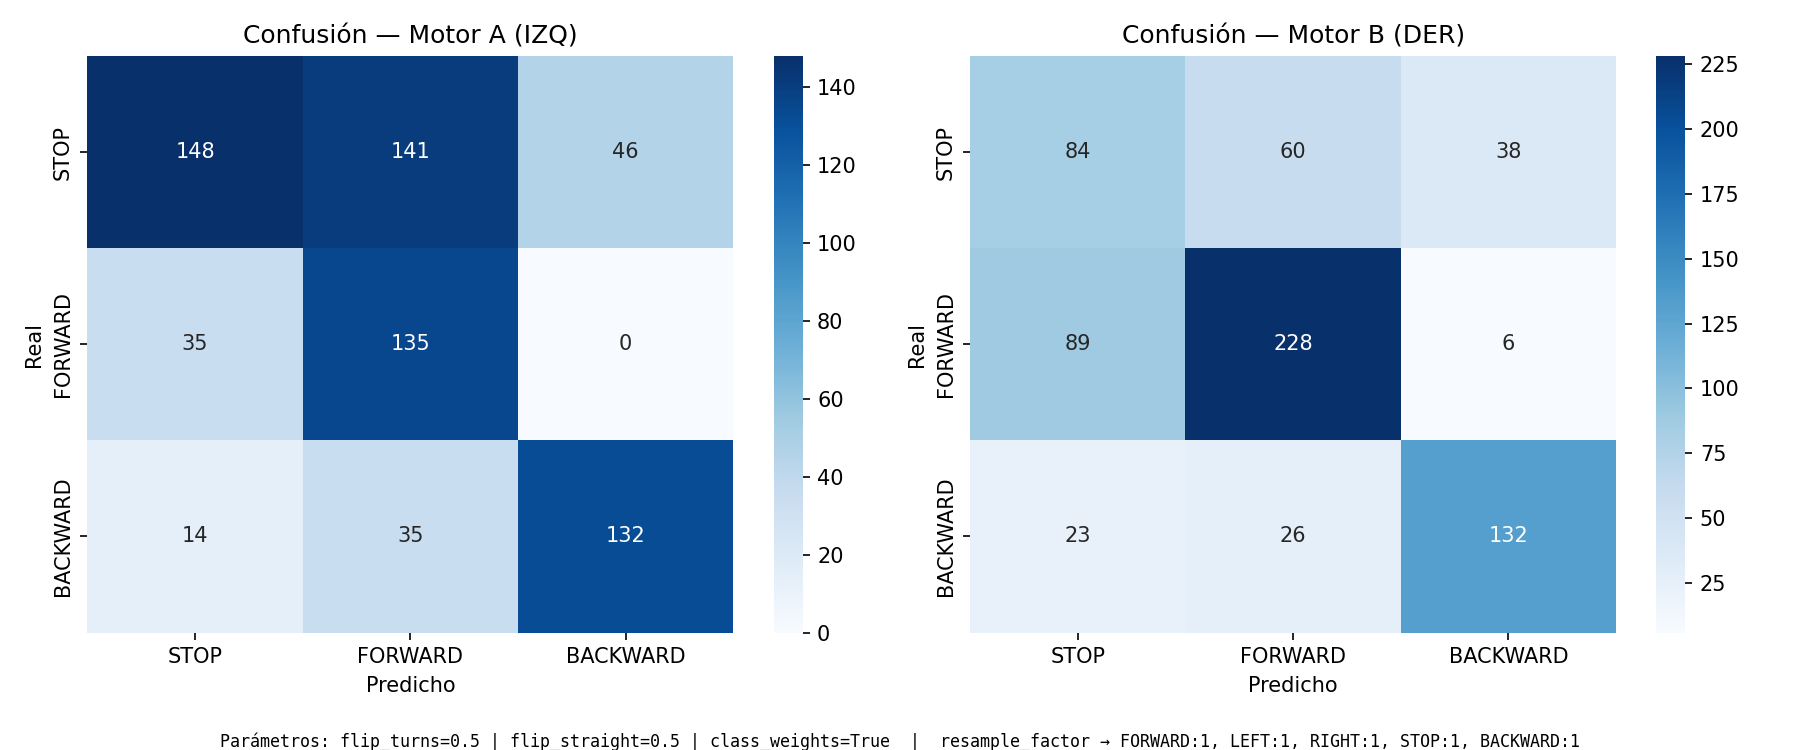
\includegraphics[width=0.72\textwidth]{../results/model_01_perframe/eval_confusion.png}
\caption{Matrices de confusión por motor del mejor modelo (model\_01, per-frame). La diagonal fuerte muestra
que clasifica bien las tres direcciones; el error dominante es STOP$\leftrightarrow$FORWARD, el borde
físicamente ambiguo desde un solo frame.}
\end{figure}

\begin{figure}[H]\centering
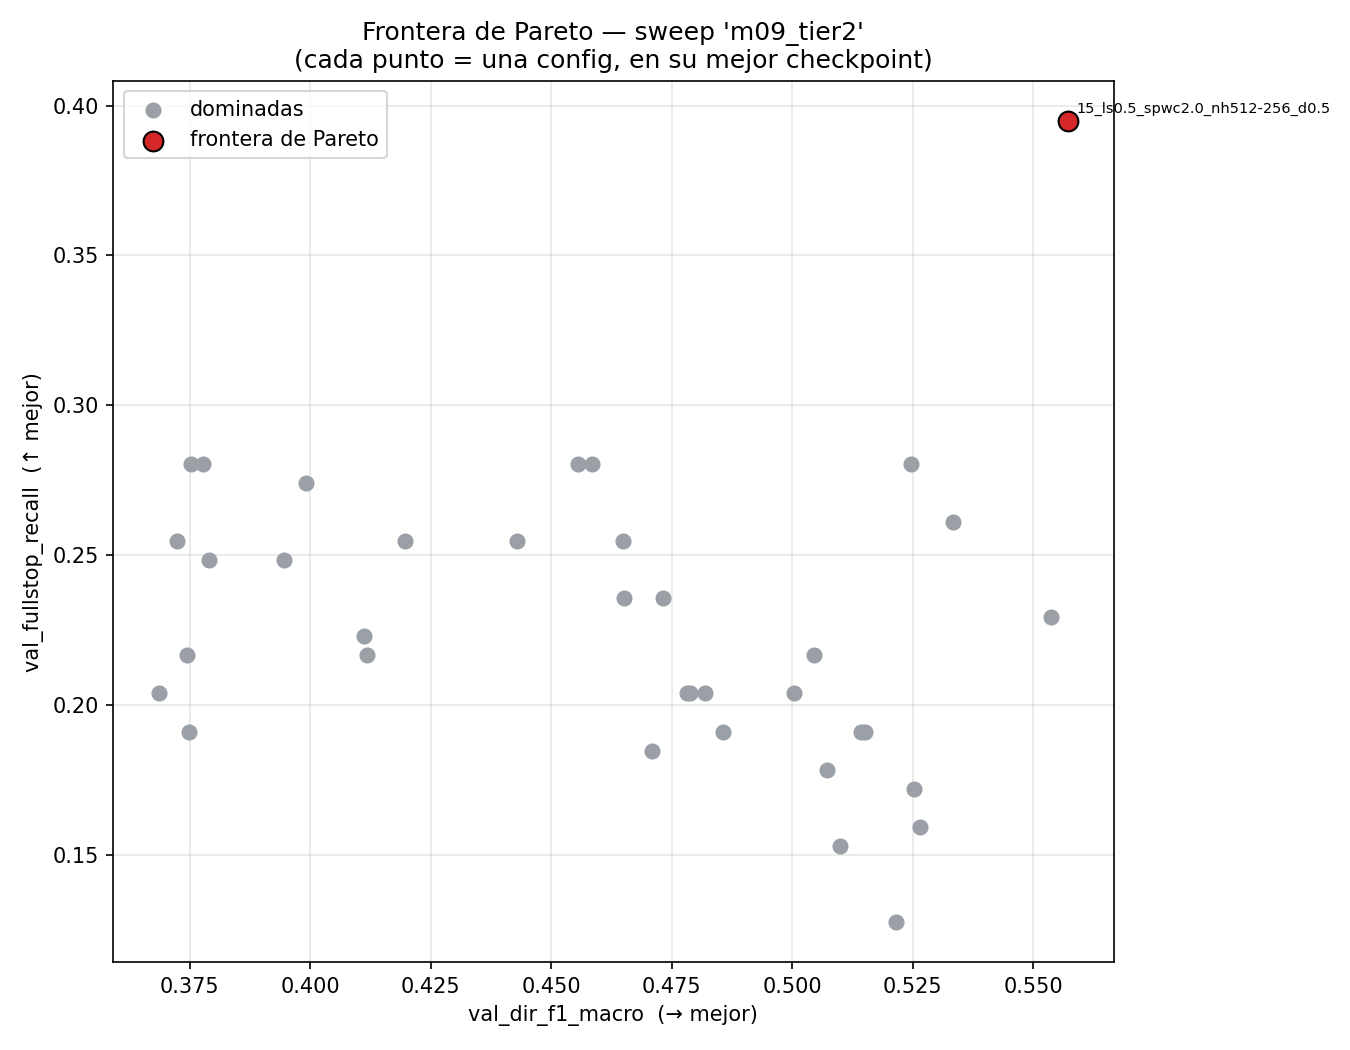
\includegraphics[width=0.7\textwidth]{../results/sweeps/m09_tier2/pareto.png}
\caption{Frontera de Pareto del sweep del híbrido (F1 macro vs recall de full-stop). Cada punto es una config
en su mejor checkpoint; en rojo, las no dominadas. La config ganadora mejora al híbrido original en ambos ejes.}
\end{figure}

\section{Conclusión: el arco completo}
El proyecto recorrió, de lo simple a lo complejo: un \textbf{baseline} tonto (RF) $\rightarrow$ el
\textbf{per-frame} (mejor) $\rightarrow$ modelos \textbf{temporales} (GRU/LSTM) $\rightarrow$ el reframe
\textbf{con signo} $\rightarrow$ el \textbf{híbrido} $\rightarrow$ y finalmente \textbf{sweeps} de los
finalistas. La conclusión es consistente y honesta:

\begin{nota}[Veredicto]
\textbf{Ningún camino superó al per-frame con clasificación explícita (model\_01, F1 0.62/0.63).} Los
temporales no aprovechan la memoria (la mayoría de las etiquetas son interpoladas: el modelo aprendería el
interpolador, no inercia real). El enfoque con signo es elegante pero rompe el STOP; el híbrido lo recupera
pero no destrona al per-frame. El sweep, exhaustivo, confirma que el per-frame ya está en su techo: tunear no
lo mueve. \textbf{El límite no es la arquitectura, es el dato} (91\% de etiquetas interpoladas, una sola
sesión, validación chica y de distribución corrida).
\end{nota}

Y un aprendizaje metodológico que vale tanto como los modelos: con una validación tan chica, \textbf{las
métricas son ruidosas}; el mecanismo de reseed mostró que varios ``ganadores'' de una sola semilla eran
casualidad. Medir con rigor (Pareto + múltiples semillas) es parte del resultado. Para el informe, esto cumple
de lleno el objetivo del enunciado de \emph{discutir las limitaciones} del enfoque.

\end{document}
